\documentclass{article}
\usepackage{amsmath, amssymb, mathtools, graphicx, fancyhdr, float}

\graphicspath{{Images/}}


\setlength{\oddsidemargin}{0in}
\setlength{\textwidth}{6.5in}
\setlength{\topmargin}{-.55in}
\setlength{\textheight}{9in}
\pagestyle{fancy}

\fancyfoot{}
\fancyhead[R]{\thepage}
\fancyhead[L]{MATH 5430}

\begin{document}
\begin{center}
    {\Huge Homework 5}
    \vspace{0.5cm}

    {\Large Michael Nameika}
\end{center}

\section*{General Linear 1st Order Systems}
\begin{itemize}
    \item[1.] (Differential calculus for matrices.) Suppose $A(t)$ and $B(t)$ are differentiable. Prove (3.77) and (3.78).
    \newline\newline
    \textit{Proof:} We begin by proving (3.77). Let $A$ be an $n\times m$ matrix and $B$ be a $m \times q$ matrix. By definition of matrix multiplication, we have
    \[[AB]_{ij} = \sum_{k = 1}^m a_{ik}b_{kj}\]
    Since derivatives of matrices are defined as term-by-term differentiation, we have that
    \begin{align*}
        \dot{[AB]}_{ij} &= \frac{d}{dt}\sum_{k = 1}^m a_{ik}(t)b_{kj}(t)\\
        &= \sum_{k = 1}^m \frac{d}{dt}a_{ik}(t)b_{kj}(t)\\
        &= \sum_{k = 1}^m (\dot{a}_{ik}(t)b_{kj}(t) + a_{ik}(t)\dot{b}_{kj}(t))\\
        &= [\dot{A}B]_{ij} + [A\dot{B}]_{ij}\\
        \implies \frac{d}{dt}AB &= \dot{A}B + A\dot{B}.
    \end{align*}
    Now, to show (3.78), notice that
    \begin{align*}
        AA^{-1} &= \mathbb{I}
    \end{align*}
    and so, let $B = A^{-1}$. Then notice
    \begin{align*}
        \frac{d}{dt} AA^{-1} &= \frac{d}{dt} AB\\
        &= \frac{d}{dt}\mathbb{I}\\
        &= \mathbf{0}.
    \end{align*}
    Thus, by the above proof, we have
    \begin{align*}
        \frac{d}{dt}AB &= \dot{A}B + A\dot{B}\\
        &= 0\\
        \implies A\dot{B} &= -\dot{A}B\\
        \implies \dot{B} &= -A^{-1}\dot{A}B\\
        \implies \dot{A^{-1}} &= -A^{-1}\dot{A}A^{-1}
    \end{align*}
    as was desired.
    \pagebreak

    \item[2.] Modify Problem 3.27 to solve the inhomogeneous initial value problem
\[\dot{x} = A(t)x(t) + f(t), \hspace{0.75cm} x(0) = x_0\]
where
\[A(t) = \begin{pmatrix}
    t & 0\\
    1 & t
\end{pmatrix}, \hspace{0.75cm} f(t) = \begin{pmatrix}
    0\\
    t
\end{pmatrix}\]
\textit{Soln.} Let us begin by solving the homogeneous problem. Note that the IVP corresponds to the following linear system:
\begin{align*}
    \dot{x}_1 &= tx_1\\
    \dot{x}_2 &= x_1 + tx_2
\end{align*}
To build the principle matrix, first consider the initial condition $x_0 = \delta_1 = (1,0)^T$. Then solving the first equation, we have
\begin{align*}
    \frac{dx_1}{dt} &= tx_1\\
    \int_{x_1(t_0)}^{x_1(t)}\frac{1}{x_1}dx_1 &= \int_{t_0}^t sds\\
    \implies \ln|x_1(t)| &= \frac{t^2}{2} - \frac{t_0^2}{2} + C\\
    \implies x_1(t) &= e^{1/2(t^2 - t_0^2)} \tag{$C = 0$ by I.C.}
\end{align*}
and so 
\begin{align*}
    \frac{dx_2}{dt} &= e^{1/2(t^2 - t_0^2)} + tx_1(t)
\end{align*}
solving the homogeneous equation gives us the same form as $x_1(t)$, but by the initial condition $\delta_1$, we have that the homogeneous solution is identically zero. For the particular solution, use the ansatz $x_{2,p} = A(t - t_0)e^{1/2(t^2 - t_0^2)}$ so that $\dot{x}_{2,p} = Ae^{1/2(t^2 - t_0^2)} + tx_{2,p}$ hence $A = 1$ and
\[x_2 = (t-t_0)e^{1/2(t^2 - t_0^2)}\]
Thus,
\[\phi_1 = \begin{pmatrix}
    e^{1/2(t^2 - t_0^2)}\\
    (t - t_0)e^{1/2(t^2 - t_0^2)}
\end{pmatrix}.\]
Now, we consider the initial condition $x_0 = \delta_2 = (0,1)^T$. From our work above, we have that $x_1(t) = 0$ and $x_2(t) = e^{1/2(t^2 - t_0^2)}$ so that
\[\phi_2 = \begin{pmatrix}
    0\\
    e^{1/2(t^2 - t_0^2)}
\end{pmatrix}.\]
Thus, our principle matrix is given
\begin{align*}
    \Pi(t,t_0) &= [\phi_1, \phi_2]\\
    &= \begin{pmatrix*}
        e^{1/2(t^2 - t_0^2)} & 0\\
        (t - t_0)e^{1/2(t^2 - t_0^2)} & e^{1/2(t^2 - t_0^2)}
    \end{pmatrix*}
\end{align*}
so that our solution is given by
\[x(t) = \begin{pmatrix}
        e^{1/2(t^2 - t_0^2)} & 0\\
        (t - t_0)e^{1/2(t^2 - t_0^2)} & e^{1/2(t^2 - t_0^2)}
\end{pmatrix}x_0\]

\[x(t) = \Pi(t,t_0)x_0 + \int_{t_0}^t\Pi(t,s)f(s)ds\]
via variation of parameters. Thus, from our work in problem 1, we have
\[x(t) = 
\begin{pmatrix}
    e^{1/2(t^2 - t_0^2)} & 0\\
    (t - t_0)e^{1/2(t^2 - t_0^2)} & e^{1/2(t^2 - t_0^2)}
\end{pmatrix}x_0 + \int_{t_0}^t \begin{pmatrix}
        e^{1/2(t^2 - s^2)} & 0\\
        (t - s)e^{1/2(t^2 - s^2)} & e^{1/2(t^2 - s^2)}
\end{pmatrix}\begin{pmatrix}
    0\\
    s
\end{pmatrix}ds\]
Notice
\begin{align*}
    \int_{t_0}^t \begin{pmatrix}
        e^{1/2(t^2 - s^2)} & 0\\
        (t - s)e^{1/2(t^2 - s^2)} & e^{1/2(t^2 - s^2)}
    \end{pmatrix}\begin{pmatrix}
        0\\
        s
    \end{pmatrix}ds &= \int_{t_0}^t \begin{pmatrix}
        0\\
        se^{1/2(t^2 - s^2)}
    \end{pmatrix}ds
\end{align*}
and that
\begin{align*}
    \int_{t_0}^t se^{1/2(t^2-s^2)}ds &= e^{1/2t^2} \int_{t_0}^t se^{-1/2s^2}ds
\end{align*}
let $u = 1/2s^2$ so that $du = sds$ and so the above integral becomes
\begin{align*}
    e^{1/2t^2} \int_{t_0}^t se^{-1/2s^2}ds &= e^{1/2t^2}\int_{1/2t_0^2}^{1/2t^2}e^{-u}du\\
    &= -e^{1/2t^2}\left[e^{-u}\right]\bigg|_{1/2t_0^2}^{1/2t^2}\\
    &=-e^{1/2t^2}\left[e^{-1/2t^2} - e^{-1/2t_0^2}\right]\\
    &= e^{1/2(t^2 - t_0^2)} - 1
\end{align*}
so that our general solution is given by
\[x(t) = \begin{pmatrix}
        e^{1/2(t^2 - t_0^2)} & 0\\
        (t - t_0)e^{1/2(t^2 - t_0^2)} & e^{1/2(t^2 - t_0^2)}
\end{pmatrix}x_0 + \begin{pmatrix}
    0\\
    e^{1/2(t^2 - t_0^2)} - 1
\end{pmatrix}\]

\end{itemize}
\section*{Reduction of Order}
\begin{itemize}
    \item[3.] Use reduction of order to find the general solution of the following equations:
    \begin{itemize}
        \item[(i)] $t\ddot{x} - 2(t + 1)\dot{x} + (t + 2)x = 0$, $\phi_1(t) = e^t$.
        \newline\newline
        \textit{Soln.} Let us begin by rewriting the differential equation as a first order system:
        \[\frac{d}{dt}\begin{pmatrix}
            x\\
            \dot{x}
        \end{pmatrix} = \begin{pmatrix}
            0 & 1\\
            -1-\tfrac{2}{t} & 2 + \tfrac{2}{t}
        \end{pmatrix}\begin{pmatrix}
            x\\
            \dot{x}
        \end{pmatrix}\]
        Since $e^t$ is a solution to the original equation, we have $\phi_1 = (e^t,e^t)^T$ is a solution to the system. Now, transforming the coordinates to $\dot{y} = X^{-1}(AX - \dot{X})y$, we have
        \[X = \begin{pmatrix}
            e^t & 0\\
            e^t & 1
        \end{pmatrix}, \hspace{0.5cm} \dot{X} = \begin{pmatrix}
            e^t & 0\\
            e^t & 0
        \end{pmatrix},\hspace{0.5cm} X^{-1} = \begin{pmatrix}
            e^{-t} & 0\\
            -1 & 1
        \end{pmatrix}\]
        so that the transformed system becomes
        \begin{align*}
            \dot{y} &= \begin{pmatrix}
                e^{-t} & 0\\
                -1 & 1
            \end{pmatrix}\left[\begin{pmatrix}
                0 & 1\\
                -t - \tfrac{2}{t} & 2 + \tfrac{2}{t}
            \end{pmatrix}\begin{pmatrix}
                e^t & 0\\
                e^t & 1
            \end{pmatrix} - \begin{pmatrix}
                e^t & 0\\
                e^t & 0
            \end{pmatrix}\right]\\
            &= \begin{pmatrix}
                e^{-t} & 0\\
                -1 & 1
            \end{pmatrix}\left[\begin{pmatrix}
                e^t & 1\\
                e^t & 2 + \tfrac{2}{t}
            \end{pmatrix} - \begin{pmatrix}
                e^t & 0\\
                e^t & 0
            \end{pmatrix}\right]\\
            &= \begin{pmatrix}
                e^{-t} & 0\\
                -1 & 1
            \end{pmatrix}\begin{pmatrix}
                0 & 1\\
                0 & 2 + \tfrac{2}{t}
            \end{pmatrix}\\
            &= \begin{pmatrix}
                0 & e^{-t}\\
                0 & 1 + \tfrac{2}{t}
            \end{pmatrix}
        \end{align*}
        So that we now have the linear system
        \begin{align*}
            \dot{y}_1 &= e^{-t}y_2\\
            \dot{y}_2 &= (1 + \tfrac{2}{t})y_2
        \end{align*}
        from the second equation, via separation of variables, we find $y_2 = t^2e^t$ and so $\dot{y}_1 = t^2$, $\implies y_1 = \tfrac{1}{3}t^3$. Converting back to $x$:
        \begin{align*}
            X\begin{pmatrix}
                \tfrac{1}{3}t^3\\
                t^2e^t
            \end{pmatrix} &= \begin{pmatrix}
                e^t & 0\\
                e^t & 1
            \end{pmatrix}\begin{pmatrix}
                \tfrac{1}{3}t^3\\
                t^2e^t
            \end{pmatrix}\\
            &=\begin{pmatrix}
                \tfrac{1}{3}t^3e^t\\
                \tfrac{1}{3}t^3e^t + t^2e^t
            \end{pmatrix}
        \end{align*}
        so that our other solution is $x_2(t) = \tfrac{1}{3}t^3e^t$ and the general solution is
        \[x(t) = C_1e^t + C_2t^3e^t\]
        


        \item[(ii)] $t^2\ddot{x} - 3t\dot{x} + 4x = 0$, $\phi_1(t) = t^2$.
        \newline\newline
        \textit{Soln.} As above, we write the differential equation as a first order system:
        \[\frac{d}{dt}\begin{pmatrix}
            x\\
            \dot{x}
        \end{pmatrix} = \begin{pmatrix}
            0 & 1\\
            -\tfrac{4}{t^2} & \tfrac{3}{t}
        \end{pmatrix}\begin{pmatrix}
            x\\
            \dot{x}
        \end{pmatrix}\]
        and since $x_1(t) = t^2$ is a solution to the differential equation, $\phi_1(t) = (t^2, 2t)^T$ is a solution to our system. Thus, transforming the coordinates, we have
        \begin{align*}
            \dot{y} &= X^{-1}(AX - \dot{X})\\
            &= \begin{pmatrix}
                \tfrac{1}{t^2} & 0\\
                -\tfrac{2}{t} & 1
            \end{pmatrix}\left[\begin{pmatrix}
                0 & 1\\
                -\tfrac{4}{t^2} & \tfrac{3}{t}
            \end{pmatrix}\begin{pmatrix}
                t^2 & 0\\
                2t & 1
            \end{pmatrix} - \begin{pmatrix}
                2t & 0\\
                2 & 0
            \end{pmatrix}\right]\\
            &= \begin{pmatrix}
                \tfrac{1}{t^2} & 0\\
                -\tfrac{2}{t} & 1
            \end{pmatrix}\left[\begin{pmatrix}
                2t & 1\\
                2 & \tfrac{3}{t}
            \end{pmatrix} - \begin{pmatrix}
                2t & 0\\
                2 & 0
            \end{pmatrix}\right]\\
            &= \begin{pmatrix}
                \tfrac{1}{t^2} & 0\\
                -\tfrac{2}{t} & 1
            \end{pmatrix}\begin{pmatrix}
                0 & 1\\
                0 & \tfrac{3}{t}
            \end{pmatrix}\\
            &= \begin{pmatrix}
                0 & \tfrac{1}{t^2}\\
                0 & \tfrac{1}{t}
            \end{pmatrix}.
        \end{align*}
        So now, we have the system 
        \begin{align*}
            \dot{y}_1 &= \tfrac{1}{t^2}y_2\\
            \dot{y}_2 &= \tfrac{1}{t}y_2.
        \end{align*}
        By separation of variables, from the second equation, we have $y_2 = t$ and so $\dot{y}_1 = \tfrac{1}{t} \implies y_1 = \ln|t|$. Transforming back to our original coordinates, we have
        \begin{align*}
            \begin{pmatrix}
                t^2 & 0\\
                2t & 1
            \end{pmatrix}\begin{pmatrix}
                \ln|t|\\
                t
            \end{pmatrix} &= \begin{pmatrix}
                t^2\ln|t|\\
                2t\ln|t| + t
            \end{pmatrix}
        \end{align*}
        so that $x_2(t) = t^2\ln|t|$ and our general solution is
        \[x(t) = C_1t^2 + C_2t^2\ln|t|.\]
    \end{itemize}
    \pagebreak
    \item[4.] Verify that the second-order equation
    \[\ddot{x} + (1 - t^2)x = 0\]
    can be factorized as 
    \[\left(\frac{d}{dt} - t\right)\left(\frac{d}{dt} + t\right)x = 0\]
    (note that the order is important.) Use this to find the solution.
    \newline\newline
    \textit{Soln.} Verifying the factorization, notice
    \begin{align*}
        \left(\frac{d}{dt} - t\right)\left(\frac{d}{dt} + t\right)x &= \left(\frac{d}{dt} - t\right)\left(\frac{dx}{dt} + tx\right)\\
        &= \frac{d}{dt}\left(\frac{dx}{dt} + tx\right) - t\left(\frac{dx}{dt} + tx\right)\\
        &= \frac{d^2x}{dt^2} + x + t\frac{dx}{dt} - t\frac{dx}{dt} - t^2x\\
        &= \frac{d^2x}{dt^2} + x - t^2x\\
        &= \ddot{x} + (1 - t^2)x.
    \end{align*}
    Now, notice that if $\left(\frac{d}{dt} + t\right)x = 0$, the differential equation is satisfied. Thus, solving this equation, we have
    \begin{align*}
        \frac{dx}{dt} + tx &= 0\\
        \implies \frac{dx}{dt} &= -tx\\
        \implies \int \frac{dx}{x} &= -\int t dt\\
        \implies \ln|x| &= -\frac{t^2}{2} + C\\
        \implies x(t) &= Ce^{-t^2/2}
    \end{align*}
    so that $x_1 = e^{-t^2/2}$ is a solution to the differential equation. Now, we write the differential equation as a linear system:
    \begin{align*}
        \frac{d}{dt}\begin{pmatrix}
            x\\
            \dot{x}
        \end{pmatrix} &= \begin{pmatrix}
            0 & 1\\
            t^2 - 1 & 0
        \end{pmatrix}\begin{pmatrix}
            x\\
            \dot{x}
        \end{pmatrix}
    \end{align*}
    Thus, $\phi_1 = (e^{-t^2/2}, -te^{-t^2/2})^T$ is a solution to the above system. Now, apply the change of coordinates $\dot{y} = X^{-1}(AX - \dot{X})y$ where
    \[X = \begin{pmatrix}
        e^{-t^2/2} & 0\\
        -te^{-t^2/2} & 1
    \end{pmatrix}, \hspace{0.4cm} A = \begin{pmatrix}
        0 & 1\\
        t^2 - 1 & 0
    \end{pmatrix}, \hspace{0.4cm} \dot{X} = \begin{pmatrix}
        -te^{-t^2/2} & 0\\
        (t^2 - 1)e^{-t^2/2} & 0
    \end{pmatrix}, \hspace{0.4cm} X^{-1} = \begin{pmatrix}
        e^{t^2/2} & 0\\
        t & 1
    \end{pmatrix}\]
    so that
    \begin{align*}
        \dot{y} &= \begin{pmatrix}
            e^{t^2/2} & 0\\
        t & 1
        \end{pmatrix}
        \left[\begin{pmatrix}
        0 & 1\\
        t^2 - 1 & 0
    \end{pmatrix}\begin{pmatrix}
        e^{-t^2/2} & 0\\
        -te^{-t^2/2} & 1
    \end{pmatrix} - \begin{pmatrix}
        -te^{-t^2/2} & 0\\
        (t^2 - 1)e^{-t^2/2} & 0
    \end{pmatrix}\right]\\
    & = \begin{pmatrix}
            e^{t^2/2} & 0\\
            t & 1
        \end{pmatrix}\left[\begin{pmatrix}
            -te^{-t^2/2} & 1\\
            (t^2 - 1)e^{-t^2/2} & 0
        \end{pmatrix} - \begin{pmatrix}
            -te^{-t^2/2} & 0\\
            (t^2 - 1)e^{-t^2/2} & 0
        \end{pmatrix}\right]\\
        &= \begin{pmatrix}
            e^{t^2/2} & 0\\
            t & 1
        \end{pmatrix}\begin{pmatrix}
            0 & 1\\
            0 & 0
        \end{pmatrix}\\
        & = \begin{pmatrix}
            0 & e^{t^2/2}\\
            0 & t
        \end{pmatrix}
    \end{align*}
    so that we have the following system:
    \begin{align*}
        \dot{y}_1 &= e^{t^2/2}y_2\\
        \dot{y}_2 &= ty_2
    \end{align*}
    and from the second equation, notice $y_2 = e^{t^2/2}$ and so 
    \[y_1 = \int_{t_0}^t e^{s^2}ds.\]
    Converting back to our original coordinates we find
    \begin{align*}
        x &= \begin{pmatrix}
            e^{-t^2/2} & 0\\
            -te^{-t^2/2} & 1
        \end{pmatrix}\begin{pmatrix}
            \int_{t_0}^t e^{s^2}ds\\
            e^{t^2/2}
        \end{pmatrix}\\
        &= \begin{pmatrix}
            e^{-t^2/2}\int_{t_0}^te^{s^2}ds\\
            -te^{-t^2/2}\int_{t_0}^te^{s^2}ds + e^{t^2/2}
        \end{pmatrix}
    \end{align*}
    so that $x_2 = e^{-t^2/2}\int_{t_0}^te^{s^2}ds$ is a solution to the system. Thus, the general solution to the differential equation is
    \[x(t) = C_1e^{-t^2/2} + C_2e^{-t^2/2}\int_{t_0}^te^{s^2}ds.\]
\end{itemize}

\pagebreak
\section*{Floquet Theory}
\begin{itemize}
    \item[5.] Compute the monodromy matrix where $A(t)$ is of period 1 and given by
    \[A(t) = \begin{cases}
        \begin{pmatrix}
            \alpha & 1\\
            0 & \alpha
        \end{pmatrix}, & 0 \leq t < \frac{1}{2},\\
        \begin{pmatrix}
            \alpha & 0\\
            1 & \alpha
        \end{pmatrix}, & \frac{1}{2}\leq t < 1,
    \end{cases} \hspace{0.5cm} \alpha \in \mathbb{C}.\]
    Note that since $A(t)$ is not continuous you have to match solutions at every discontinuity such that the solutions are continuous. 
    

    
    For which values of $\alpha$ remain all solutions bounded? Show that the bound found in problem 3.31 is optimal by considering $A(t/T)$ as $T \to 0$.
    

    
    (Note that we could approximate $A(t)$ by continuous matrices and obtain the same qualitative result with an arbitrary small error.)
    \newline\newline
    \textit{Soln.} For $0\leq t < \tfrac{1}{2}$, we have 
    \[A(t) = \begin{pmatrix}
        \alpha & 1\\
        0 & \alpha
    \end{pmatrix}\]
    is constant for these values of $t$, we have $\Pi(t,t_0) = e^{(t - t_0)A}$, so that 
    \[\Pi(t,t_0) = \begin{pmatrix}
        e^{(t - t_0)\alpha} & (t-t_0)e^{(t - t_0)\alpha}\\
        0 & e^{(t - t_0)\alpha}
    \end{pmatrix} \hspace{0.5cm} t \in [0, \tfrac{1}{2}).\]
    
    For $\tfrac{1}{2} \leq t < 1$, since 
    \[\begin{pmatrix}
        \alpha & 0\\
        1 & \alpha
    \end{pmatrix}^T = \begin{pmatrix}
        \alpha & 1\\
        0 & \alpha
    \end{pmatrix}\]
    and that $\exp(A^T) = (\exp(A))^T$, we have
    \[\Pi(t,t_0) = \begin{pmatrix}
        e^{(t - t_0)\alpha} & 0\\
        (t - t_0)e^{(t - t_0)\alpha} & e^{(t - t_0)\alpha}
    \end{pmatrix}, \hspace{0.5cm} t \in [\tfrac{1}{2},1).\]
    Now, since the monodromy matrix is defined as
    \[m(t_0) = \Pi(t_0 +T,t_0) = \Pi(1,0)\]
    we use the fact that 
    \[\Pi(t,t_1) = \Pi(t,t_0)\Pi(t_0,t_1)\]
    to find
    \begin{align*}
        \Pi(1,0) &= \Pi(1,\tfrac{1}{2})\Pi(\tfrac{1}{2},0)\\
        &= \begin{pmatrix}
            e^{(1 - \tfrac{1}{2})\alpha} & 0\\
            (1 - \tfrac{1}{2})e^{(1 - \tfrac{1}{2})\alpha} & e^{(1 - \tfrac{1}{2})\alpha}
        \end{pmatrix}\begin{pmatrix}
            e^{\tfrac{1}{2}\alpha} & \tfrac{1}{2}e^{\tfrac{1}{2}\alpha}\\
            0 & e^{\tfrac{1}{2}\alpha}
        \end{pmatrix}\\
        &= \begin{pmatrix}
            e^{\alpha} & \tfrac{1}{2}e^{\alpha}\\
            \\
            \tfrac{1}{2}e^{\alpha} & \tfrac{5}{4}e^{\alpha}
        \end{pmatrix}
    \end{align*}
    thus
    \[m(t_0) = \begin{pmatrix}
        e^{\alpha} & \tfrac{1}{2}e^{\alpha}\\
        \\
        \tfrac{1}{2}e^{\alpha} & \tfrac{5}{4}e^{\alpha}
    \end{pmatrix}.\]
    Now, to find the values of $\alpha \in \mathbb{C}$ for which solutions remain bounded, we find the Floquet multipliers, that is the eigenvalues of the monodromy matrix:
    \begin{align*}
        \left|\begin{matrix}
            e^{\alpha} - \lambda & \tfrac{1}{2}e^{\alpha}\\
            \\
            \tfrac{1}{2}e^{\alpha} & \tfrac{5}{4}e^{\alpha} - \lambda
        \end{matrix}\right| &= (e^{\alpha} - \lambda)(\tfrac{5}{4}e^{\alpha} - \lambda) - \tfrac{1}{4}e^{2\alpha}\\
        &= \lambda^2 - \lambda e^{\alpha} - \tfrac{5}{4}\lambda e^{\alpha} + \tfrac{5}{4}e^{2\alpha} - \tfrac{1}{4}e^{2\alpha}\\
        &= \lambda^2 - \tfrac{9}{4}\lambda e^{\alpha} + e^{2\alpha}\\
        &= 0\\
        \implies \lambda_{\pm} &= \frac{\tfrac{9}{4}e^{\alpha} \pm \sqrt{\tfrac{81}{16}e^{2\alpha} - 4e^{2\alpha}}}{2}\\
        &= \frac{\tfrac{9}{4}e^{\alpha} \pm \sqrt{\tfrac{17}{16}e^{2\alpha}}}{2}\\
        &= e^{\alpha} \left(\frac{9}{8} \pm \frac{\sqrt{17}}{8}\right).
    \end{align*}
    Recall that if $|\lambda| \leq 1$, we have that the system is stable, hence bounded. Now, let $\alpha = a + ib$ for $a,b \in \mathbb{R}$ and let $x = \tfrac{9}{8} + \tfrac{\sqrt{17}}{8}$ and $y = \tfrac{9}{8} - \tfrac{\sqrt{17}}{8}$.
    Notice that $x,y > 0$ since $9 > \sqrt{17}$. Looking case by case, notice
    \begin{align*}
        |\lambda_+| &= |e^{a + ib}x| \leq 1\\
        \implies e^a &\leq \frac{1}{x}\\
        \implies a &\leq -\ln(x) \tag{$\ln(\cdot)$ monotone}\\
        \text{Re}(\alpha) &\leq -\ln(x)
    \end{align*}
    similarly, for $\lambda_-$, we have
    \begin{align*}
        |\lambda_-| &= |e^{a + ib}y| \leq 1\\
        \implies e^a &\leq \frac{1}{y}\\
        \implies a &\leq -\ln(x) \tag{$\ln(\cdot)$ monotone}\\
        \text{Re}(\alpha) &\leq -\ln(x).
    \end{align*}
    Thus, since $x > y$, and $\ln(\cdot)$ is monotone, we have that 
    \[\text{Re}(\alpha) \leq -\ln\left(\frac{9}{8} + \frac{\sqrt{17}}{8}\right)\]
    will guarantee stability. To show the bound in problem 3.31 is optimal, consider $A(t/T):$
    \[A(t/T) = \begin{cases}
        \begin{pmatrix}
            \alpha & 1\\
            0 & \alpha
        \end{pmatrix}, & 0 \leq \frac{t}{T} < \frac{1}{2},\\
        \begin{pmatrix}
            \alpha & 0\\
            1 & \alpha
        \end{pmatrix}, & \frac{1}{2} \leq \frac{t}{T} < 1
    \end{cases}, \hspace{0.4cm} \alpha \in \mathbb{C}\]
    which we may rewrite as
    \[A(t/T) = \begin{cases}
        \begin{pmatrix}
            \alpha & 1\\
            0 & \alpha
        \end{pmatrix}, & 0\leq t < \frac{T}{2}\\
        \begin{pmatrix}
            \alpha & 0\\
            1 & \alpha
        \end{pmatrix}, & \frac{T}{2} \leq t < T
    \end{cases}, \hspace{0.4cm} \alpha \in \mathbb{C}\]
    which has principle matrix solutions
    \[\Pi(\tfrac{T}{2},0) = \begin{pmatrix}
        e^{\tfrac{T}{2}\alpha} & \tfrac{T}{2}e^{\tfrac{T}{2}\alpha}\\
        0 & e^{\frac{T}{2}\alpha}  
    \end{pmatrix}\]
    and
    \[\Pi(T,\tfrac{T}{2}) = \begin{pmatrix}
        e^{\tfrac{T}{2}\alpha} & 0\\
        \tfrac{T}{2}e^{\tfrac{T}{2}\alpha} & e^{\tfrac{T}{2}\alpha}
    \end{pmatrix}\]
    and notice that for any $t$, $\text{eig}\left(\frac{A + A^*}{2}\right) = \text{Re}(\alpha)$. Thus, by the bound in problem 3.31, we have
    \[\|\Pi(t,t_0)\| \leq e^{(t - t_0)\text{Re}(\alpha)}\]
    to show a bound for the operator norm is optimal, usually you find a norm 1 vector and take their product and find the norm of that product. For this, I have no idea how to do that without a specific norm, and I have no idea how to use $A(t/T)$.
    

    
    \pagebreak
    


    \item[6.] Numerically solve the Mathieu equation (3.148). Re-create the stability diagram in figure 3.6 on page 96.
    \[\ddot{x} = -\omega^2(1 + \varepsilon\cos(t))x.\]
    To begin, we rewrite this differential equation as a system:
    \begin{align*}
        \frac{d}{dt}\begin{pmatrix}
            x\\
            \dot{x}
        \end{pmatrix} &= \begin{pmatrix}
            0 & 1\\
            -\omega^2(1 + \varepsilon\cos(t))x & 0
        \end{pmatrix}
        \begin{pmatrix}
            x\\
            \dot{x}
        \end{pmatrix}
    \end{align*}
    to numerically solve this, we implemented RK4 in MATLAB for fixed values of $\omega, \varepsilon$ and solved for the initial conditions $\delta_1 = (1,0)^T$, $\delta_2 = (0,1)^T$ on the interval $[0,2\pi]$. At the value $2\pi$, we take the associated solutions for $x$ and $\dot{x}$ corresponding to $\delta_1$ and $\delta_2$ and build the monodromy matrix to find the value of $\Delta$ ($\Delta = \text{tr}(m(t_0))/2$). By varying $\omega$ and $\varepsilon$ and computing $\Delta$, we find the following stability diagram:
    \begin{figure}[H]
        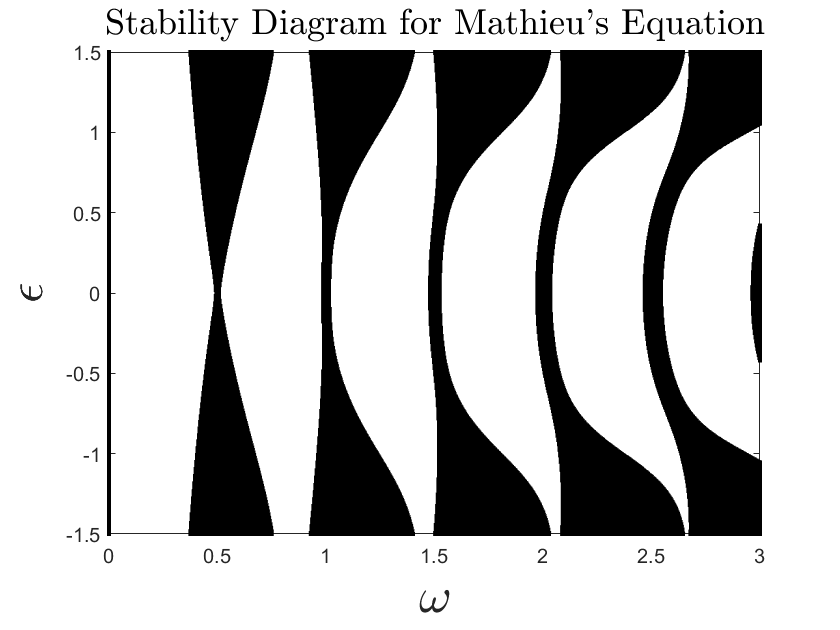
\includegraphics[scale = 0.35]{mathieu_stability_fine.png}
        \centering
        \caption{Stability region for Mathieu's equation. Dark region corresponds to $|\Delta| \geq 1$, light regions correspond to $|\Delta| < 1$, as in the textbook.}
    \end{figure}
    
\end{itemize}


\end{document}
